\documentclass[activite]{thedocument}
\usepackage{texmaths-tikz}
\usepackage{tabularray}
\startdatakeys
\source{}
\cycle{}
\competencesDuSocle{}
\connaissancesRequises{}
\competencesTravaillees{}
\enddatakeys
\begin{document}
\begin{enumerate}
    \item Sur quelles figures a-t-on coloriés le quart de la longueur du segment ou de la surface ?
    \def\coloract{Rainbow1-bleu}
    \vspace{0.5cm}
    \begin{center}
    \begin{tabular}{c c c}
    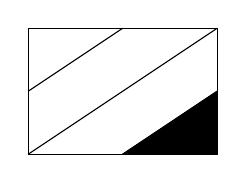
\begin{tikzpicture}[scale=0.8]
    \def\rectwidth{3}
    \def\rectheight{2}
    \coordinate(A)at(0,0);
    \coordinate(B)at(\rectwidth,0);
    \coordinate(C)at(\rectwidth,\rectheight);
    \coordinate(D)at(0,\rectheight);
    \path(A)--(B)coordinate[pos=0.5](E);
    \path(B)--(C)coordinate[pos=0.5](F);
    \path(C)--(D)coordinate[pos=0.5](G);
    \path(D)--(A)coordinate[pos=0.5](H);
    \filldraw[fill=\coloract](E)--(B)--(F)--cycle;
    \draw(A)rectangle(C);
    \draw(E)--(F);
    \draw(A)--(C);
    \draw(H)--(G);
    \end{tikzpicture}
    &
    \begin{tikzpicture}[scale=0.8]
    \def\y{0.15}
    \draw(0,0)--(5,0);
    \foreach\x in{0,1,...,5}{
    \draw(\x,-\y)--(\x,\y);
    }
    \draw[red](2,0)--(3,0);
    \end{tikzpicture}
    &
    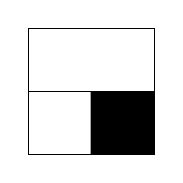
\begin{tikzpicture}[scale=0.8]
    \def\cote{2}
    \coordinate(A)at(0,0);
    \coordinate(B)at(\cote,0);
    \coordinate(C)at(\cote,\cote);
    \coordinate(D)at(0,\cote);
    \coordinate(O)at(\cote/2,\cote/2);
    \path(A)--(B)coordinate[pos=0.5](E);
    \path(B)--(C)coordinate[pos=0.5](F);
    \path(A)--(D)coordinate[pos=0.5](G);
    \fill[\coloract](E)--(B)--(F)--(O)--cycle;
    \draw(A)rectangle(C);
    \draw(F)--(G);
    \draw(E)--(O);
    \end{tikzpicture}
    \\
    figure 1&figure2&figure3
    \\
    &&
    \\
    &
    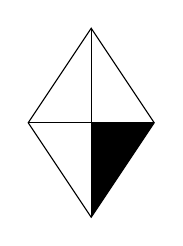
\begin{tikzpicture}[scale=0.8]
        \def\loswidth{2}
        \def\losheight{3}
        \coordinate(O)at(0,0);
        \coordinate(A)at(0,-\losheight/2);
        \coordinate(C)at(0,\losheight/2);
        \coordinate(B)at(\loswidth/2,0);
        \coordinate(D)at(-\loswidth/2,0);
        \fill[\coloract](A)--(B)--(O)--cycle;
        \draw(A)--(B)--(C)--(D)--cycle;
        \draw(A)--(C);
        \draw(B)--(D);
    \end{tikzpicture}
    &\\
    &figure4&
    \end{tabular}
    \end{center}
    \vspace{0.5cm}
    \item Sur quelles figures a-t-on colorié les deux-tiers de la surface ?
    \vspace{0.5cm}
    \begin{center}
        \begin{tabular}{c c c c}
        \begin{tikzpicture}[scale=0.8]
        \coordinate(O)at(0,0);
        \coordinate(A)at(90:1);
        \coordinate(B)at(162:1);
        \coordinate(C)at(232:1);
        \coordinate(D)at(304:1);
        \coordinate(E)at(376:1);
        \fill[Rainbow1-bleu](O)--(16:1)arc(16:162:1)--cycle;
        \draw(O)circle(1);
        \foreach\X in{A,B,...,E}{
        \draw(O)--(\X);
        }
        \end{tikzpicture}
        &
        \begin{tikzpicture}[scale=0.8]
        \def\y{0.2}
        \coordinate(A)at(0,0);
        \path(-1,0)--(A)([turn]80:3)coordinate(B);
        \path(A)--(B)coordinate[pos=1/3](C);
        \path(A)--(B)coordinate[pos=2/3](D);
        \path(A)--(C)([turn]90:\y)coordinate(C1);
        \path(A)--(C)([turn]-90:\y)coordinate(C2);
        \path(A)--(D)([turn]90:\y)coordinate(D1);
        \path(A)--(D)([turn]-90:\y)coordinate(D2);
        \draw(A)--(B);
        \draw[red](A)--(D);
        \draw(C1)--(C2);
        \draw(D1)--(D2);
        \end{tikzpicture}
        &
        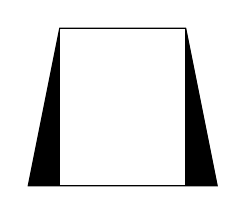
\begin{tikzpicture}[scale=0.8]
            \def\uwidth{2}
            \def\dwidth{3}
            \def\height{2.5}
            \coordinate(A)at(-\dwidth/2,0);
            \coordinate(B)at(+\dwidth/2,0);
            \coordinate(C)at(+\uwidth/2,\height);
            \coordinate(D)at(-\uwidth/2,\height);
            \coordinate(E)at(-\uwidth/2,0);
            \coordinate(F)at(\uwidth/2,0);
            \fill[\coloract](A)--(B)--(C)--(D)--cycle;
            \fill[white](E)rectangle(C);
            \draw(A)--(B)--(C)--(D)--cycle;
            \draw(E)--(D);
            \draw(F)--(C);
        \end{tikzpicture}
        &
        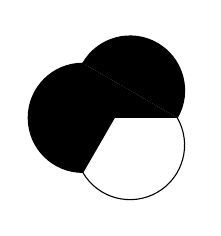
\begin{tikzpicture}[scale=0.8]
            \def\radius{0.866}
            \coordinate(O)at(0,0);
            \coordinate(A1)at(0:1);
            \coordinate(A2)at(120:1);
            \coordinate(A3)at(240:1);
            \path(A1)--(A2)coordinate[pos=0.5](B1);
            \path(A2)--(A3)coordinate[pos=0.5](B2);
            \path(A3)--(A1)coordinate[pos=0.5](B3);
        
            \draw[fill=\coloract](A1)arc[start angle=-30,delta angle=180,radius=\radius];
            \draw[fill=\coloract](A2)arc[start angle=90,delta angle=180,radius=\radius];
            \draw(A3)arc[start angle=210,delta angle=180,radius=\radius];
            \fill[\coloract](A1)--(A2)--(O)--cycle;
            \fill[\coloract](A2)--(A3)--(O)--cycle;
            \foreach\i in{1,2,3}{
                \draw(O)--(A\i);
            }
        \end{tikzpicture}\\
        figure 5&figure6&figure7&figure8
        \end{tabular}
    \end{center}
    \vspace{0.5cm}
    \item Quelle fraction des fleurs de ce bouquet représentent les fleurs rouges.
    \vspace{0.5cm}
    \end{enumerate}
    \begin{center}
        \pdf[scale=0.6]{6eme_Ch4_A2-bouquet}
    \end{center}
\end{document}